\subsubsection{距離センサー}\label{distance}
\begin{table}[H]
	\begin{tabular}{|p{\colF}|p{\colG}|} \hline
	名称 & 距離センサー(きょりせんさー)\\ \hline
	接続箇所 & アナログコネクタ (3pin)\\ \hline
	機能概要 & センサーから障害物までの距離を計測\\ \hline
  \end{tabular}
\end{table}

\begin{table}[H]
	\begin{tabular}{|p{\colF}|p{\colG}|}	\hline
	サンプルコードの場所 & ome/05/anain.hsp\\ \hline
	raspiへの入力 & 距離をあらわす0から1023の値。測定可能な距離は10cmから80cm。\\ \hline
	raspiへの入力方法 & val = spiget(ピン番号, チャンネル番号)\\ \hline
	raspiからの出力 & なし\\ \hline
	raspiからの出力方法 & なし\\ \hline
  \end{tabular}
\end{table}

\begin{table}[H]
	\begin{tabular}{|p{\colF}|p{\colG}|} \hline
	使い道 & 距離計測、障害物センサーとして。\\ \hline
	注意事項 & レンズを覗き込むと目に影響を及ぼすことがあるため覗き込まないこと。\\ \hline
	補足 & 入力の単位はセンチメートルではないため、変換が必要です。出力は0から1023で出力されるので、これを数式\ref{eq:distance}で変換する必要があります。数式\ref{eq:distance}の$x$にセンサーからのデータを代入することでセンチメートルへの変換が可能です。
	\begin{equation}
	 -\frac{1}{36} \times \frac{5000}{1023}x + \frac{845}{9}
	 \label{eq:distance}
	\end{equation}
三角測量の原理により、ある三角形があったとき一辺の長さとそれに対する角の角度がわかれば三角形が決定します(余弦定理)。距離センサーは光源と受光器で成っています。受光器は光源が反射してきた光の位置を計測することが出来ます。光源と受光器は固定されているので、その間の距離と対する角の角度がわかり、これと三角関数を使うと距離が求まります\\ \hline
  \end{tabular}
\end{table}

\begin{figure}[H]
	\begin{tabular}{|p{\colH}|p{\colI}|p{\colH}|p{\colI}|} \hline
	外観 & 
	\begin{minipage}[t]{\linewidth}
    \smallskip
      \centering
      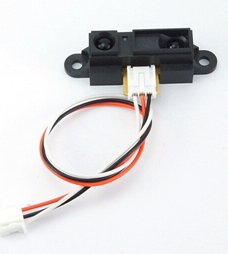
\includegraphics[width=\linewidth]{images/chap05/text05-img031.png}
      \caption{距離センサー}
      \smallskip
    \end{minipage} &
    回路記号 & 回路記号はありません。\\ \hline
  \end{tabular}
\end{figure}